\question{Câu 10}

 Thiết kế mạch dao động tạo sóng vuông đối xứng có chu kỳ $100\,\textsf{kHz}$, chỉ dùng 1 OPAMP, các điện trở và tụ.

\answer{a}{Thiết kế mạch}

Ta có, $F=100\,\textsf{kHz } \Rightarrow \textsf{ } T = 10\,\textsf{us}$, xem xét schematic và đồ thị như hình dưới:

\begin{figure}[H]
	\centering
	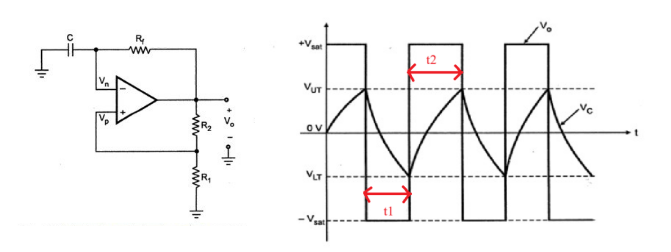
\includegraphics[width=\linewidth]{./my-chapters/my-images/Question10/C10_Hình1.png}
	\caption{Schenatic và đồ thị điện áp ngõ ra theo thời gian.}
\end{figure}

\begin{itemize}[label=-]
	\item Giả sử ban đầu $V_c$ và $V_o = 0$, nhờ vào độ lệch điên áp ngõ vào $V_{os}$, $V_o$ có giá trị tiến lên $V_{sat}$ hoặc $-V_{sat}$.
	\item Ta giả sử $V_o = V_{sat}$  \\ [3pt]
	$\Rightarrow$  $V_c = V_n$ bắt đầu nạp điện tích lên $V_{sat}$ với thời gian $\tau = R_f.C$.
	\item $v_p = \dfrac{R_2}{R_1 + R_2} V_{sat} = B V_{sat} = V_{UT}$  \\ [3pt]
	$\Rightarrow$  Trong quá trịnh $V_c$ tích điện lến $V_{sat}$, nếu $V_c < v_p$ \\ [3pt]
	$\Rightarrow$  $v_o$ vẫn duy trì ở $V_{sat}$, nếu $V_c > v_p$  \\ [3pt]
	$\Rightarrow$  $v_o = -V_{sat}$.
	\item Khi $v_o = -V_{sat}$  $\Rightarrow$  $v_p = \dfrac{-R_2}{R_1 + R_2} V_{sat} = -B V_{sat} = V_{UL}$  \\ [3pt]
	$\Rightarrow$  $V_c$ bắt đầu xả điện tích về 0 và tiếp tục nạp điện tích đến $-V_{sat}$  \\ [3pt]
	$\Rightarrow$  Trong quá trình $V_c$ từ  $\dfrac{R_2}{R_1 + R_2} V_{sat}$  xuống  $-V_{sat}$, nếu $V_c > v_p$  $\Rightarrow$  $v_o$ vẫn duy trì ở  $-V_{sat}$, nếu $V_c < v_p$  \\ [3pt]
	$\Rightarrow$  $v_o =  V_{sat}$.
\end{itemize}

\begin{itemize}[label=-]
	\item Xét khoảng thời gian $t_1$ :\\ [3pt]
	$V_c(t) = -V_{sat} + \left(V_{UT}-(-V_{sat})\right) e^{-t/R_fC }$  $\Rightarrow$  $-BV_{sat}=  -V_{sat} + (BV_{sat}+V_{sat}) e^{-t_1/R_fC}$ \\ [3pt]
	$\Rightarrow$  $-BV_{sat}=  -V_{sat} + (1+B)V_{sat} e^{-t_1/R_fC}$ $\Rightarrow$ $(1-B)V_{sat} = (1+B)V_{sat} e^{-t_1/R_fC}$ \\ [3pt]
	$\Rightarrow e^{-t_1/R_fC} =  \dfrac{1-B}{1+B}$ $\Rightarrow$ $t_1 = R_f .C \ln \left(\dfrac{1+B}{1-B}\right)$
	
	\item Xét khoảng thời gian $t_2$ :\\ [3pt]
	$V_c(t) = V_{sat} + ( V_{LT}-V_{sat}) e^{-t/R_fC}$  $\Rightarrow$  $BV_{sat}=  V_{sat} + (-BV_{sat}-V_{sat}) e^{-t_2/R_fC}$ \\ [3pt]
	$\Rightarrow$  $(1-B)V_{sat} = (1+B)V_{sat} e^{-t_2/R_fC}$ \\ [3pt]
	$\Rightarrow e^{-t_2/R_fC} =  \dfrac{1-B}{1+B}$ $\Rightarrow$ $t_2 = R_f .C \ln \left(\dfrac{1+B}{1-B}\right)$ \\ [3pt]
	$\Rightarrow T = t_1 + t_2 = 2 R_f .C \ln \left(\dfrac{1+B}{1-B}\right)$
\end{itemize}

Ta chọn $R_1 = R_2 = R_f = 1k$ $\Rightarrow$  $10\mu = 2 \times 1k \times C \ln(3)$  $\Rightarrow$  $C = 4.5\,\text{nF}$.

Để cho opamp tạo mạch vuông chuẩn ta chỉnh giá trị \finalresult{SlewRate = 1000M(V/s)}.

\answer{b}{Mô phỏng mạch dùng Multisim (hoặc các chương trình tương tự).}

\begin{figure}[H]
	\centering
	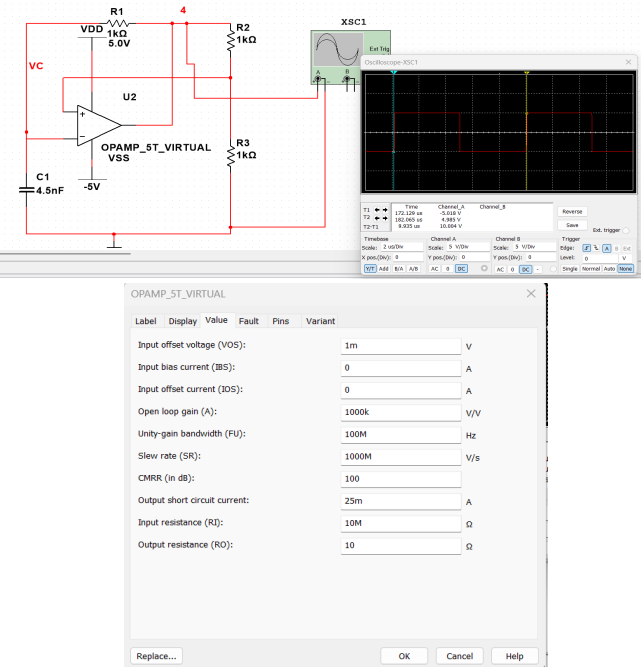
\includegraphics[width=\linewidth]{./my-chapters/my-images/Question10/C10_Hình2.png}
	\caption{Mô phỏng Multisim.}
\end{figure}